\documentclass{article}

\usepackage{cite}
\usepackage[square, comma, numbers, sort&compress]{natbib}
\usepackage{wrapfig}
\usepackage[utf8]{inputenc}
\usepackage[T1]{fontenc}
\usepackage{lmodern}
\usepackage{amsfonts}
\usepackage{amsmath}
\usepackage{graphicx}
\usepackage{booktabs}
\usepackage{placeins}
% \usepackage{pdfpages}
\usepackage{caption}
\usepackage{multirow}
\usepackage{hhline}
\usepackage{capt-of}
\usepackage{array}
\usepackage{subcaption}
\usepackage{here}
\usepackage[labelfont=bf, format=plain, font=it]{caption}
\usepackage[german]{babel}

\parindent=0pt

\begin{document}






\section{Wechselwirkung von Teilchen mit Materie}
\graphicspath{{bilder/1-1/}}
	\subsection{Wechselwirkung von geladenen Teilchen}
		\FloatBarrier

Nur die elektromagnetische Wechselwirkung ist von Bedeutung. Folgende Reaktionen führen zu einem
Energieverlust von geladenen Teilchen in Materie:

\begin{itemize}
  \item Ionisation der Atome im Detektormaterial
  \item Anregung der Atome im Detektormaterial
  \item Bremsstrahlung (relevant für Elektronen/Positronen)
  \item \v{C}erenkov-Strahlung
  \item Übergangsstrahlung
\end{itemize}

% \[-\left(\frac{dE}{dx}\right)_{\text{tot}} = -\left(\frac{dE}{dx}\right)_{\text{coll}}
% -\left(\frac{dE}{dx}\right)_{\text{rad}} -\left(\frac{dE}{dx}\right)_{\text{pair}}
% -\left(\frac{dE}{dx}\right)_{\text{photo}} -\left(\frac{dE}{dx}\right)_{\text{compt}}
% -\left(\frac{dE}{dx}\right)_{\text{kal}}-\ldots\]
 
 Beispiel: Gesamte Energieverlustrate $-\frac{dE}{dx}$ für Myonen in Kupfer (s. Abb.
 \ref{myonenInKupfer)}). Der Großteil wird durch die Bethe-Bloch-Formel beschrieben (Herleitung
 erfolgt im nächsten Kapitel).
Unterschiedliche Energie der Projektile führt über unterschiedliche Wechselwirkung zum
Energieverlust.

\begin{align*}
-\left(\frac{\mathrm{d}E}{\mathrm{d}x}\right)_{\text{tot}} &= -\left(\frac{\mathrm{d}E}{\mathrm{d}x}\right)_{\text{coll}}
-\left(\frac{\mathrm{d}E}{\mathrm{d}x}\right)_{\text{rad}} -\left(\frac{\mathrm{d}E}{\mathrm{d}x}\right)_{\text{pair}}
-\left(\frac{\mathrm{d}E}{\mathrm{d}x}\right)_{\text{photo}} -\left(\frac{\mathrm{d}E}{\mathrm{d}x}\right)_{\text{compt}} \\
&\hspace{4mm} -\left(\frac{\mathrm{d}E}{\mathrm{d}x}\right)_{\text{kal}}-\ldots
\end{align*}
 
\begin{figure}
	\centering
	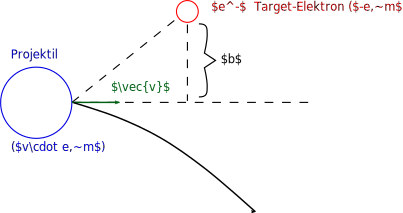
\includegraphics[width=0.5\textwidth]{bethebloch.jpg}
 	\caption{Energieverlust von Myonen in Kupfer}
 	\label{myonenInKupfer}
\end{figure}

\begin{figure}
	\centering
	\includegraphics[width=0.5\textwidth]{bethebloch2.jpg}
	\caption{$\frac{dE}{dx}$-Kurven für verschiedene Teilchen (gemessen in der
	PEP4/9-TPC)}
	\label{}
\end{figure}
 
 Beachte: $\frac{dE}{dx}$ für "`schwere"' Teilchen (z.B. $\alpha$) wird in diesem Impulsbereich gut
 durch die Bethe-Bloch-Formel beschrieben. Der Energieverlust durch Ionisation und Anregung von
 Targetelektronen dominiert. $\frac{dE}{dx}$ für Elektronen/Positronen folgt jedoch nicht der
 Bethe-Bloch-Formel!
 
 \FloatBarrier
			\subsubsection{Bethe-Bloch-Formel}
				Zur klassischen Herleitung der Bethe-Bloch-Formel betrachten wir den Energieverlust $\frac{dE}{dx}$
eines schweren (d.h. $m>>m_e$), geladenen Teilchens durch Streuung an einem Hüllenelektron eines
Targetatoms.
\\
Dabei gelten folgende Annahmen:
\begin{itemize}
  \item das Hüllenelektron ist in Ruhe (Vernachlässigung der Bahnbewegung und des Rückstoßes),
  \item der Energieübertrag ist sehr viel größer als die Bindungsenergie eines Hüllenelektrons.
\end{itemize}


{\Huge ZEICHNUNG}

Der Impulsübertrag ist das Zeitintegral der durch das elektrische Feld des Projektils auf das
Target einwirkenden Kraft. Für die longitudinalen bzw. transversalen Komponenten des E-Feldes gilt

\[E_l(-x)=-E_l(x)~~~~~~~~~~~~~~~~~~~E_t(-x)=E_t(x)\]

d.h. nur der Transversalanteil ist wichtig, die longitudinalen Komponenten im Impulsübertrag heben
sich auf. Es gilt daher

\[\Delta p= \int_{-\infty}^{\infty}F\cdot dt = \int_{-\infty}^{\infty}eE_t\cdot dt =
e\int_{-\infty}^{\infty}E_t\frac{dt}{dx}\cdot dx
=e\int_{-\infty}^{\infty}E_t\frac{1}{v}\cdot dx
=\frac{e}{v}\int_{-\infty}^{\infty}E_t\cdot dx\]

Mit Gauß $\int_{-\infty}^{\infty}E_t2\pi bdx=4\pi ze$ folgt

\[\Delta p = \frac{2ze^2}{vb}\]

und somit für den Energieübertrag

\[\Delta E=\frac{\Delta p^2}{2m_e}=\frac{2z^2e^4}{m_ev^2b^2} .\]

Eine Elektronendichte von $n_e$ ergibt daher einen Energieverlust von 

\[-dE(b)=\Delta E(b)n_edv=\frac{2z^2e^4}{m_ev^2b^2}n_e2\pi b db dx\]

Nach der Integration von $b_min$ bis $b_max$ erhält man daraus:

\[-\left(\frac{dE}{dx}\right)=\frac{4\pi z^2
e^4}{m_ev^2}n_e\text{ln}\left(\frac{b_{\text{max}}}{b_{\text{min}}}\right)\]

Nun müssen nur noch $b_{\text{min}}$ bis $b_{\text{max}}$ abgeschätzt werden. $b_{\text{min}}$ wird über das
kinematische Limit abgeschätzt: Eine frontale Kollision liefert den maximalen Energieübertrag

\[\Delta E_{\text{max}}=\frac{1}{2}m_e(2v)^2\gamma^2.\]

Mit der oben abgeleiteten Beziehung

\[\Delta E(b)=\frac{2z^2e^4}{m_ev^2b^2}\overset{!}{=}\Delta E_{\text{max}}\]

ergibt sich daraus:

\[b_{\text{min}}=\frac{ze^2}{\gamma m_e v^2}.\]

Die Abschätzung von $b_{\text{max}}$ folgt aus der "`adiabatischen Invarianz"': Die Targetelektronen
sind in Atomen gebunden und "`umkreisen"' die Atomkerne mit einer mittleren Orbitalfrequenz
$\overline{\nu}$. Damit ein Energieübertrag stattfindet, muss die Zeitdauer der Störung, $\Delta t$,
kürzer sein als die Periodendauer $\tau$:

\[\Delta t=\frac{b}{\gamma v} \le \tau =\frac{1}{\overline{\nu}}\]

Daraus folgt

\[b_{\text{max}}=\frac{\gamma v}{\overline{\nu}}.\]

Jetzt führen wir noch eine Größe for die Elektronen-Dichte des Target-Materials ein:

\[n_e=N_A\cdot \rho\cdot \frac{Z}{A}\]

mit der Avogadrozahl $N_A$, der Targetdichte $\rho$, der Ordnungszahl $Z$ und der Massenzahl $A$.
Einsetzen der Grenzen für den Stoßparameter in die Formel und Substitution von $n_e$ führt zu

\[-\left(\frac{dE}{dx}\right)_{\text{coll}} = \frac{4\pi z^2e^4}{m_ev^2}N_A\cdot \rho
\frac{Z}{A}\cdot\text{ln}\left(\frac{\gamma^2 m_e v^3}{2e^2\overline{\nu}}\right), \]

was der klassischen Formel von Bohr entspricht. Diese beschreibt den Energieverlust für schwere
Teilchen (Protonen, $\alpha$-Teilchen,\ldots) durch Anregung und Ionisation. Für leichte Teilchen
müssen Quanteneffekte berücksichtigt werden.
\\
Die quantenmechanische Rechnung führt zur Bethe-Bloch(-Sternheimer)-Formel:

\[-\left(\frac{dE}{dx}\right)_{\text{coll}} = 2\pi N_A r_e^2 m_e c^2 \rho \frac{Z}{A}
\frac{z^2}{\beta^2}\left[ \text{ln} \left( \frac{2m_e c^2 \gamma^2 \beta^2 W_{\text{max}}}{I^2}
\right) -2\beta^2 -\delta -2\frac{c}{z} \right]\]

mit 

\[\beta =
\frac{v}{c},~~~~~~~~~~~~\gamma=\frac{1}{\sqrt{1-\beta^2}}~~~~~~~~~~~~
r_e=\frac{1}{4\pi\epsilon_0}\cdot\frac{e^2}{m_e c^2}\]

sowie
\begin{description}
\item[$z$]Ladung des einfallenden Teilchens
\item[$Z, A$] Ordnungs- und Massenzahl des Targets
\item[$\rho$] Targetdichte
\item[$N_A$] Avogradozahl
\item[$I$] mittleres Ionisationspotential (Materialkonstante des Targets)
\item[$W_{\text{max}}$] max. Energieübertrag in einer Einzelkollision
\item[$\delta$] Dichtekorrektur (Polarisationseffekt, $\delta \approx 2\text{ln}(\gamma)+K$)
\item[$c$] Schalenkorrektur (wichtig für kleine Projektilgeschwindigkeiten)
\end{description}


Anmerkungen zur Bethe-Bloch-Formel:
\begin{itemize}
  \item sie beschreibt den Energieverlust sehr gut im Bereich $0,1 < \gamma\beta < 100$;
  \item es gibt drei Bereiche:
  			\begin{itemize}
  			  \item bei niedrigen Energien gibt es einen Abfall bis zu einem Minimum (bei $\gamma\beta$
  			  ca. 3-3,5), Teilchen an diesem Punkt sind minimal ionisierende Teilchen;
  			  \item danach beginnt ein logarithmischer Anstieg mit zunehmender Teilchenenergie, der
  			  sogenannte "`relativistische Anstieg"';
  			  \item bei hohen Energien wird das Fermi-Plateau erreicht: durch Polarisationseffekte erreicht
  			  der Energieverlust  einen Sättigungswert (Dichtekorrektur);
  			  \end{itemize}
  \item beim Energieverlust handelt es sich um einen statistischen Vorgang.
\end{itemize}

Die Bethe-Bloch-Formel beschreibt den mittleren Energieverlust durch Ionisation und Anregung. Sie
gilt für alle geladenen Teilchen außer Elektronen und Positronen. Für diese muss die Gleichheit der
Massen und die Ununterscheidbarkeit der Stoßpartner berücksichtigt werden. Unsere Ableitung
unterscheidet sich von der Bethe-Bloch-Formel numerisch durch einen Faktor 2, was durch eine
mangelhafte Berücksichtigung von Fernstößen zustande kommt. Für die quantenmechanische Beschreibung
des Energieverlustes gibt es verschiedene Varianten der $\frac{dE}{dx}$-Formel, was an der
unterschiedlichen Parametrisierung der Fernstöße, d.h. jenes Energieverlustes, bei dem die Bindung
der Elektronen in den Atomhüllen nicht vernachlässigbar ist.
\\
Meist wird der Energieverlust pro Wegstrecke $\frac{1}{\rho}\frac{dE}{dx}$ angegeben, wobei $\rho$
die Dichte in $\frac{\text{g}}{\text{cm}^3}$ ist. $\frac{1}{\rho}\frac{dE}{dx}$ ist für ein MIP nur
schwach vom Absorbermaterial abhängig und beträgt ca. 

\[2 \text{MeV}\frac{\text{cm}^2}{\text{g}}.\]
			\subsubsection{Landau-Verteilung}
				Wie kann die Energieverteilung des Energieverlustes beschrieben werden? Der Energieverlust ist ein
statistischer Prozess mit einer asymmetrischen Verteilungsfunktion, da Kollisionen mit kleinem
Energieübertrag wahrscheinlicher sind als solche mit großen Energieübetrag.

\begin{figure}[H]
	\centering
	\includegraphics[width=0.5\textwidth]{landau.jpg}
	\caption{Die Energieverteilung des Energieverlustes ist eine Landau-Verteilung.}
	\label{}
\end{figure}

Die Ausläufer bei hohen Energieüberträgen kommt von (selten auftretenden) Kollisionen mit kleinen
Stoßparametern, wobei Elektronen mit großen Energien (keV), sogenannte $\delta$-Elektronen,
freigesetzt werden. Die Asymmetrie kommt daher, dass der mittlere Energieverlust höher
ist als der wahrscheinlichste Energieverlust.
\\
Bei dünnen Absorbern wird der Energieverlust durch eine Landau-Verteilung beschrieben, bei dicken
Absorbern geht diese über in eine Gauß-Verteilung.
			\subsubsection{Bragg-Kurve}
				Wie tief dringen Teilchen in das Detektormaterial ein? Man kann für jede
Projektil/Target-Kombination nur eine mittlere Eindringiefe angeben. 
			\subsubsection{Delta-Elektronen}
				\FloatBarrier

Die kinetischen Energien der Elektronen ist proportional zu $\frac{1}{\Delta E^2}$.
$\Delta E$ ist dabei der Energieübertrag des Projektils auf das Hüllenelektron.

\[\frac{d\sigma}{d\Delta E} = \frac{2\pi\cdot z^2\cdot \alpha^2\cdot \hbar^2}{\beta^2\cdot m_e}\cdot
\frac{1}{\Delta E^2}
\]

Die Ausläufer dieser Verteilung gehen bis $\Delta E_\text{max}$,

\[\Delta E_\text{max} = \frac{2m_e\cdot c^2\cdot \beta^2\cdot \gamma^2}{1+ 2\,\gamma\,
\frac{m_e}{M}+\left( \frac{m_e}{M} \right)^2}\]

mit den Grenzwerten
\begin{itemize}
  \item $\gamma\rightarrow\infty$: $\Delta E_\text{max} \rightarrow \gamma Mc^2$
  \item $m_e = M$: $\Delta E_\text{max} =m_e c^2 (\gamma -1) = E- m_e c^2$ \\
  		Die komplette Energie wird auf das Hüllenelektron übertragen.
\end{itemize}

Für relativistische Teilchen ($\gamma >> 1$) kann $\Delta E_\text{max}$ sehr groß werden und
Elektronen mit Energien von einigen keV hervorbringen. In Detektoren mit hoher Granularität und Ortsauflösung (z.B.
Blasenkammern) können sie als sogenannte Delta-Elektronen nachgewiesen werden.
\\
Seltene Abstrahlung hoher Energie führt auch zu größeren Fluktuationen in $\frac{\mathrm{d}E}{\mathrm{d}x}$-Messungen
zur Teilchenidentifikation und damit zu einer schlechteren Auflösung. Auch bei Detektoren mit
geringer Granularität führt die Abstrahlung von Delta-Elektronen zu einer schlechteren
Ortsauflösung.
\\
Eine genaue Rechnung zeigt: 

\[\Delta E (\Theta) = \frac{2\,m_e}{\text{tan}^2\Theta} \]

Größere Abstrahlungswinkel führen zu kleineren Energien der Delta-Elektronen, was in einer
geringeren Reichweite resultiert.
\FloatBarrier
			\subsubsection{Energieverlust von Elektronen und Positronen}
				\FloatBarrier
Elektronen und Positronen haben durch ihre geringe Masse eine Sonderstellung
($m_{e^{\pm}} \approx 511$~keV/c$^2$, $m_{\mu} \approx 106$~MeV/c$^2$). Zusätzlich zum Energieverlust durch Ionisation und
Anregung hat daher der Energieverlust durch Bremsstrahlung eine größere Bedeutung:

\[-\left(\frac{\mathrm{d}E}{\mathrm{d}x}\right)_{\text{tot}} = -\left(\frac{\mathrm{d}E}{\mathrm{d}x}\right)_{\text{coll}}
-\left(\frac{\mathrm{d}E}{\mathrm{d}x}\right)_{\text{rad}} \]

Beim Energieverlust durch Ionisation und Anregung muss die Bethe-Bloch-Formel wegen der geringen
Masse modifiziert werden, aber auch, da eine Kollision zwischen quantenmechanisch nicht
unterscheidbaren Teilchen stattfindet. Die Ionisationsverluste steigen logarithmisch mit $E$ und
linear mit $Z$, die Bremsstrahlungsverluste dagegen in etwa linear mit $E$ und quadratisch mit $Z$.
Für hohe Energien (> 1~GeV) ist die Bremsstrahlung der dominierende Prozess.

\begin{figure}
	\centering
	\includegraphics[width=0.5\textwidth]{energieverlust.jpg}
	\caption{}
	\label{}
\end{figure}

% Elektronen/Positronen Streuung an Targetelektronen fällt unter Ionisation, wenn der Energieübertrag
% pro Kollision unter 0,255~MeV liegt und unter M\o ller-Streuung (Bhabha-Streuung), wenn er darüber
% liegt.

\FloatBarrier
			\subsubsection{Bremsstrahlung}
				Bremsstrahlung wird emittiert, wenn (hochenergetische) geladene Teilchen in einem äußeren
elektrischen Feld abgelenkt werden, beispielsweise im Coulomb-Feld eines Atomkerns oder eines
Hüllenelektrons des Targets.
\\
Die zughörigen Feyman-Diagramme niedrigster Ordnung:
\\
\\

% \begin{fmffile}{diagram}
% \begin{fmfgraph}(40,25)
% \fmfleft{i1,i2}
% \fmfright{o1,o2}
% \fmf{photon}{i1,v1,o1}
% \fmf{fermion}{i2,v2,o2}
% \fmf{photon}{v1,v2}
% \end{fmfgraph}
% \end{fmffile} 


% \begin{fmffile}{hilde}
% \begin{fmfgraph}(40,25)
% \fmfleft{i1,i2}
% \fmfright{o1,o2}
% \fmf{fermion}{i2,v2,v1,o1}
% \fmf{photon}{i1,v1}
% \fmf{photon}{v2,o2} 
% \end{fmfgraph}
% \end{fmffile} 



\begin{minipage}[t]{0.3\textwidth}
\begin{fmffile}{hubert}
\begin{fmfgraph*}(100,100)
\fmfleft{i1,i2}
\fmfright{o1,o2}
\fmf{fermion}{i1,v1,v2,o2}
\fmf{photon}{i2,v2}
\fmf{photon}{v1,o1}
\fmflabel{v1}{v1}
\fmflabel{v2}{v2}
% \fmflabel{$e^-(p)$}{i1}
% \fmflabel{$\gamma(k)$}{i2}
% \fmflabel{$\gamma(k)$}{o1}
% \fmflabel{$e^-(p)$}{o2}
\end{fmfgraph*}
\end{fmffile}
\end{minipage}
% \begin{minipage}[t]{0.3\textwidth}
% \begin{fmffile}{hubert}
% \begin{fmfgraph}(100,100)
% \fmfleft{i1,i2}
% \fmfright{o1,o2}
% \fmf{fermion}{i1,v1,v2,o2}
% \fmf{photon}{i2,v2}
% \fmf{photon}{v1,o1}
% \fmflabel{$v_1$}{v1}
% \fmflabel{$v_2$}{v2}
% % \fmflabel{$e^-(p)$}{i1}
% % \fmflabel{$\gamma(k)$}{i2}
% % \fmflabel{$\gamma(k)$}{o1}
% % \fmflabel{$e^-(p)$}{o2}
% \end{fmfgraph}
% \end{fmffile}
% \end{minipage}


\subsubsection*{Energieverlust durch Bremsstrahlung}

Für hohe Energien kann der Energieverlust durch Bremsstrahlung angenähert weren durch:

\[-\left(\frac{dE}{dx}\right)_{\text{rad}} = 4\alpha \rho N_A \cdot \frac{Z(Z+1)}{A} \cdot z^2\cdot
\left(\frac{1}{4\pi \epsilon_0} \frac{e^2}{mc^2} \right)^2 \cdot E\cdot \text{ln}(183\cdot
Z^{-\frac{1}{3}}) \]

Der Beitrag $Z^2$ kommt von der Ablenkung im Feld des Kerns mit der Ladung $Z\cdot e$, der Beitrag
$Z$ von der Ablenkung im Feld der $Z$ Hüllenelektronen jeweils mit Ladung $-e$. Hierbei wird nicht
berücksichtigt, dass die Hüllenelektronen das Feld des Atomkerns teilweise abschirmen und die Formel
daher nur für große $E$ gültig ist.
\\
Beachte: Bereits für ds zweitleichteste Teilchen, das Myon, ist der Bremsstrahlungsverlust 40.000
mal kleiner als für das Elektron. 

\[-\left(\frac{dE}{dx}\right)_{\text{rad}} \sim E~~~~~~~~~~\text{und}~~~~~~~~~
-\left(\frac{dE}{dx}\right)_{\text{rad}} \sim \frac{1}{m^2}\]

\subsubsection*{Kritische Energie $E_c$}

Die kritische Energie ist jene Energie eines Projektils, bei welcher der Energieverlust durch
Strahlung gleich dem Energieverlust durch die Kollision ist:

\[-\left(\frac{dE}{dx}\right)_{\text{rad}} \bigg|_{E_c} = -\left(\frac{dE}{dx}\right)_{\text{coll}}
\bigg|_{E_c}  \]

$E_c$ ist abhängig von der Teilchenart des Projektils und vom Targetmaterial (wenn nicht anders
gekennzeichnet, beziehen sich Literaturwerte auf Elektronen). Die kritische Energie skaliert in etwa
mit dem Quadrat der Projektilmasse. Um nun beispielsweise die kritische Energie für Myonen zu
erhalten, verwendet man:

\[E_c^\mu = E_c^e \left( \frac{m_\mu}{m_e} \right)^2 \]

Zur groben Abschätzung von $E_c$ sind diverse Näherungen gegeben, z.B.

\[E_c = \frac{800}{Z+1{},2}~\text{MeV} \]

oder für Festköper

\[E_c = \frac{610}{Z+1{,}24}~\text{MeV} \]

oder für Gase

\[E_c = \frac{710}{Z+0{,}92}~\text{MeV} \]


Die bekannten Zahlenwerte für $E_c$ schwanken relativ stark:

\begin{figure}[H]
	\centering
	\includegraphics[width=0.5\textwidth]{tabelle1.jpg}
	\caption{}
	\label{}
\end{figure}

\subsubsection*{Strahlungslänge $\chi_0$}

Die Strahlungslänge ist jene Strecke, in der die Energie des Projektils durch Strahlungsverlust um
einen Faktor $\frac{1}{e}(\approx)$63,2\% kleiner wird:

\[E(x)=E_0\cdot e^{-\frac{x}{\chi_0}}\]

Diese Beziehung ist nur sinnvoll für Energien größer als $E_c$. Die Literaturwerte für $\chi_0$
beziehen sich dabei stets auf Elektronen, für andere Teilchen skaliert die Strahlungslänge mit dem
Quadrat der Projektilmasse (ebenso wie bei $E_c$).
\\
Die oben gegebene Formel für die Bremsstrahlung führt für die Elektronen auf eine Strahlungslänge
von 

\[\frac{1}{\chi_0}=4\cdot\alpha \rho N_A \cdot\frac{Z(Z+1)}{A}\cdot
r_e^2\cdot\text{ln}\left(183\cdot Z^{-1/3}\right)\]

\[\text{Näherungsformel:}~~\chi_0\bigg[\frac{\text{g}}{\text{cm}^2}\bigg] \approx
180~\frac{A}{Z^2}\] 

Meist werden Materialdicken von Targets in Einheiten von $\chi_0$ angegeben, womit der
Strahlungsverlust pro Targetdicke dann materialunabhängig ist. Genauso wird die Strahlungslänge -
analog zur Energieverlustrate - auf die Targetdichte bezogen ($\rho \chi_0\rightarrow\chi_0$) und
folglich in [g/cm$^2$] angegeben:

\begin{figure}[H]
	\centering
	\includegraphics[width=0.5\textwidth]{tabelle2.jpg}
\end{figure}





\end{document}